\documentclass{article}

% Language setting
% Replace `english' with e.g. `spanish' to change the document language
\usepackage[english]{babel}

% Set page size and margins
% Replace `letterpaper' with `a4paper' for UK/EU standard size
\usepackage[letterpaper,top=2cm,bottom=2cm,left=3cm,right=3cm,marginparwidth=1.75cm]{geometry}

% Useful packages
\usepackage{amsmath}
\usepackage{graphicx}
\usepackage[colorlinks=true, allcolors=blue]{hyperref}

\title{Report For Assignment One}
\author{Jawad Ahmed(20P-0165) \ Section: BCS-6A}

\begin{document}
\maketitle

\section{Introduction}

The purpose of the assignment is to get started with Python programming, and get to know about the Google Colab and it's connectivity with Google Drive.

The assignment is about text processing. We have to calculate the Automated Readability Index(ARI) of all the files present in the given directory. 

\section{Explanation of Assignment}

\subsection{How sentences are defined and python code for counting sentences}

On each occurrence of a period, colon, semicolon, question mark and exclamation marks are all counted as a sentence. 

Python code for counting sentences is shown in Fiqure 1.
\subsubsection{Explanation of counting sentences code}
I have saved all the given characters whose occurance will be counted as a sentence in a python list. The function will take content of the file as function parameter. Then I have looped over the sentence terminators list and started counting each characters occurances in the file content with the help of built-in count function and added all the character occurances in the total sentences variable and returned it at the end. 

\begin{figure}
\centering
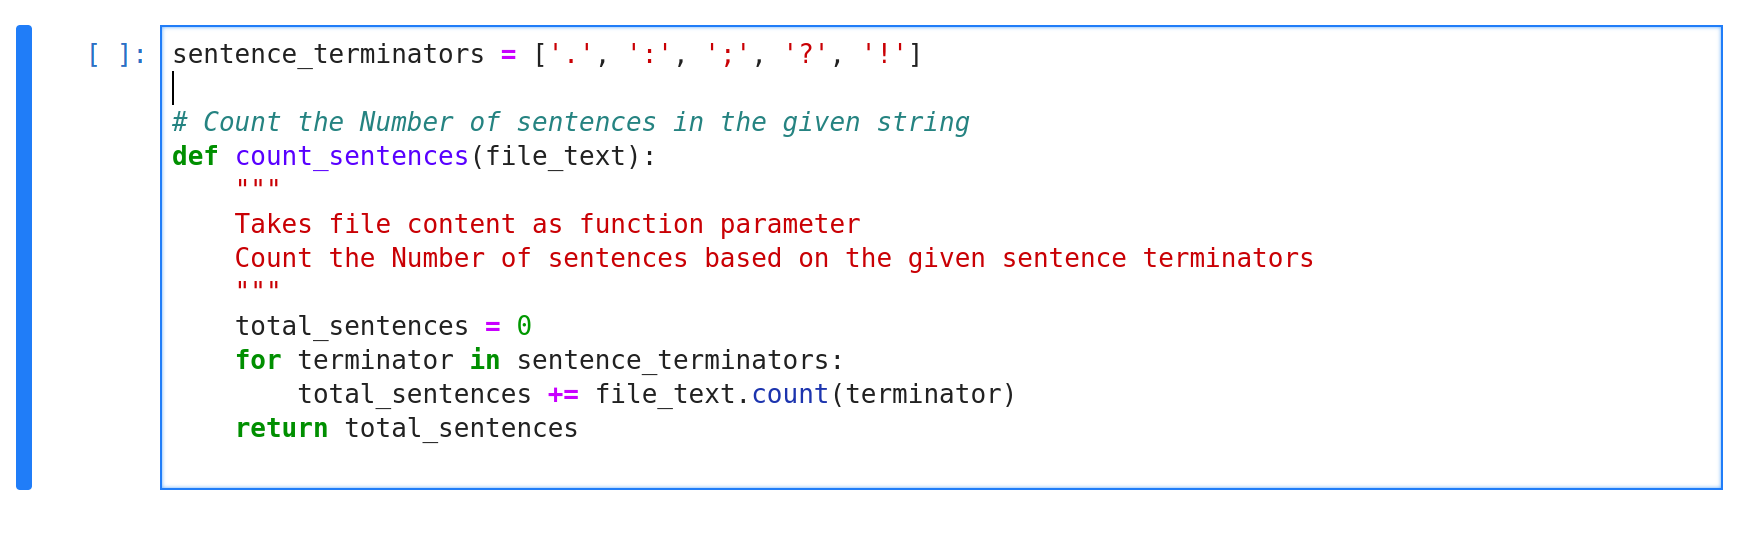
\includegraphics[scale=0.2]{screenshots/ai_a1-1.png}
\caption{\label{fig:python_code_counting_sentences}Python code for counting sentences}
\end{figure}

\subsection{How words are defined and python code for counting words}

A word is sequence of one or more alpha-numeric characters delimited by white
space or by a sentence terminators as discussed above, whether or not it is an actual English word. White space is defined as a space, tab, a new line character, and the end of the string itself. Any continuous sequence of alphabets and digits is considered as a word.

Python code for counting words is shown in Figure 2. 
\subsubsection{Explanation of counting words code}
Frist of all I have defined words terminators in the python list that includes some words terminators and also sentence terminators occurance also used to identify words. 

Second I have defined the countwords function that will be going to take file content as a function parameter. The countwords function algorithm is:
\begin{enumerate}
  \item Make file content string to list (every character will be list item).
  \item Loop over the complete list and if the word terminator found then replace word terminator with hash sign.
  \item After doing the above two steps join the string back.
  \item Then split the string based on hash sign.
  \item Then count that elements of the list that are not empty (those are words).
\end{enumerate}

\begin{figure}
\centering
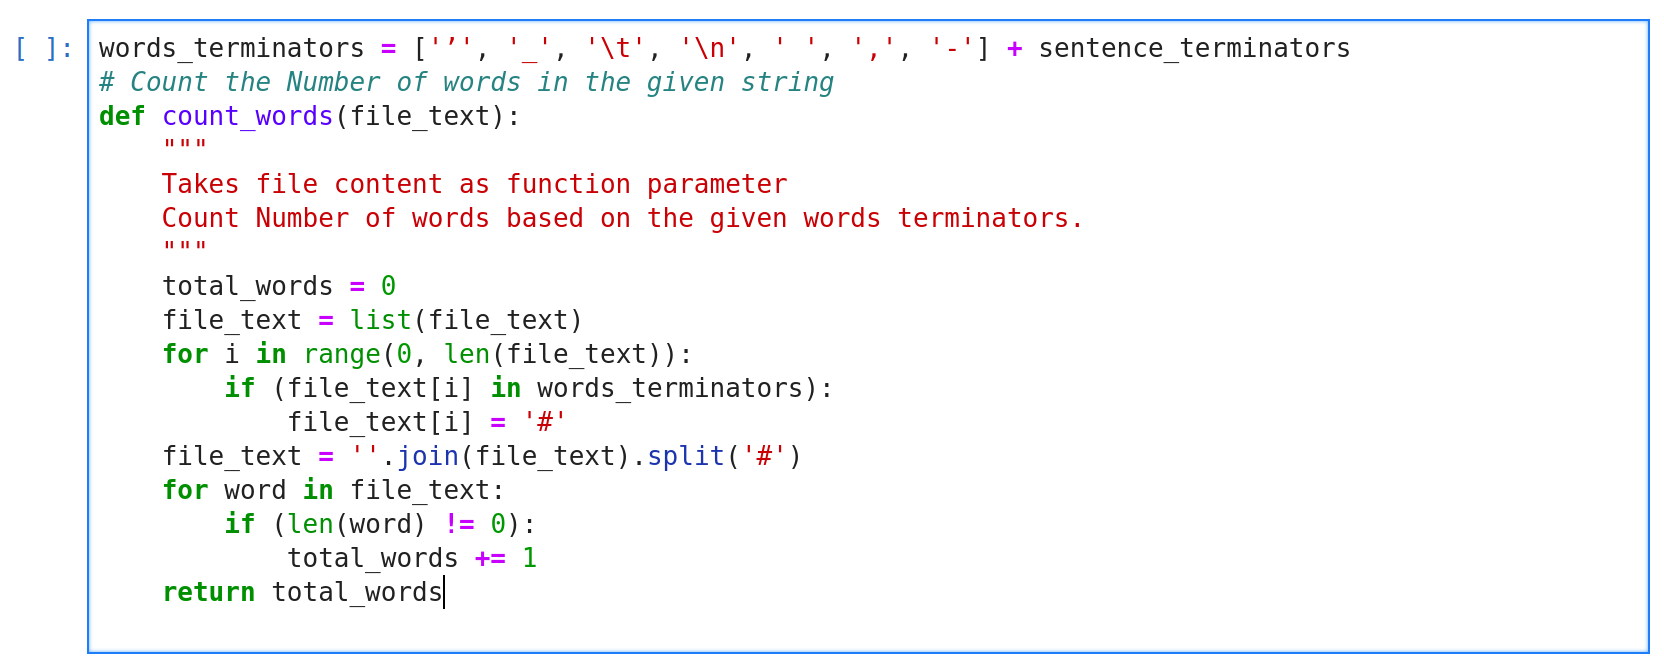
\includegraphics[scale=0.2]{screenshots/ai_a1-2.png}
\caption{\label{fig:python_code_counting_words}Python code for counting words}
\end{figure}

\subsection{How characters are defined and python code for counting characters}

All the characters except for the words and sentence terminators will be counted as a character. The python code for counting characters is shown in Figure 3.

\begin{figure}
\centering
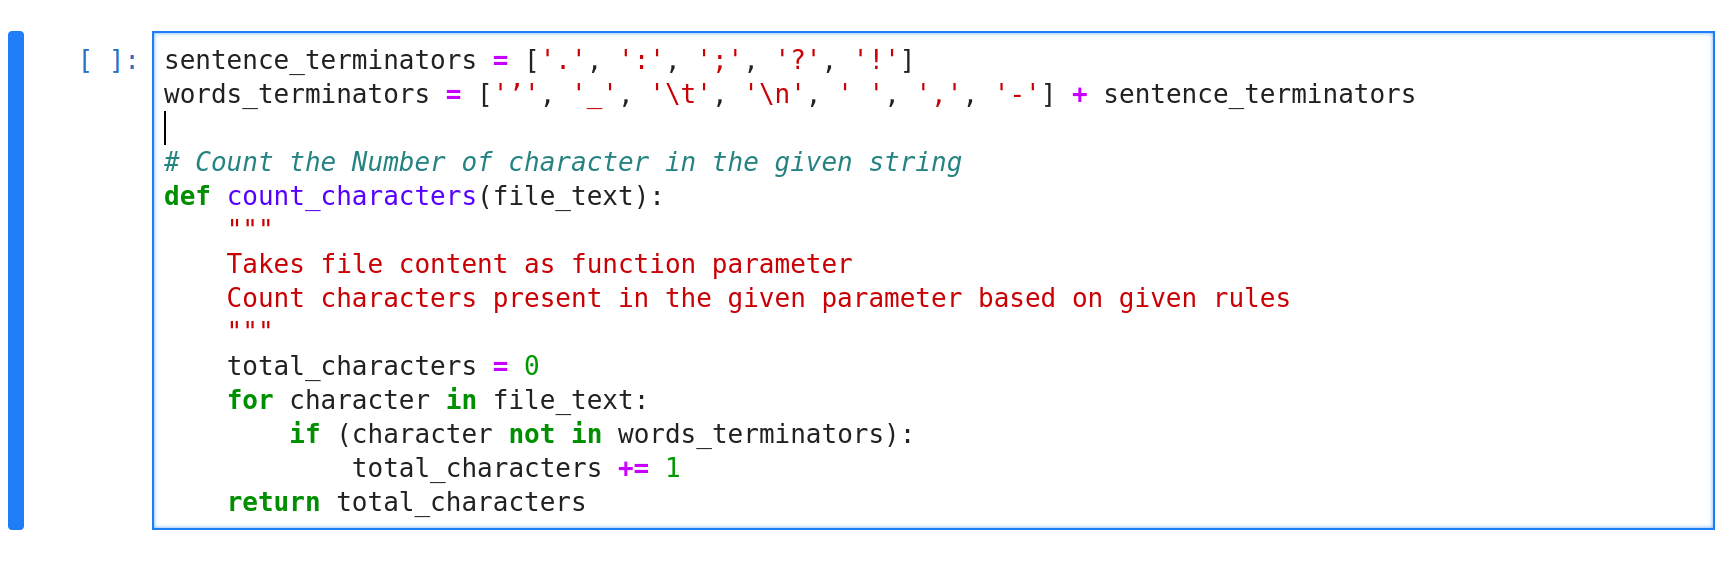
\includegraphics[scale=0.2]{screenshots/ai_a1-3.png}
\caption{\label{fig:python_code_counting_characters}Python code for counting characters}
\end{figure}

\subsubsection{Explanation of counting characters code}

The counting words function will be going to take file content as a function parameter. The algorithm for counting character is simple. Loop over the given file content string and if that character is not present in words and sentence terminator list then increment total characters by one. At the end of the for loop return the total character variable that has the result.





\subsection{Calculating Automated Readability Index(ARI)}
Automated Readability Index(ARI) is a score designed to gauge the readability of a text, and can be used as a feature for developing models for text authorship.
\

The formula for calculating ARI is:

\[ 
  4.71 \left( \frac{characters}{words} \right) + 0.5  \left( \frac{words}{sentences} \right) - 21.43
\]

Python code for calculating ARI shown in Figure 4.


\subsubsection{Explanation of Automated Readability Index(ARI) Code}

The function take no of characters, no of words, no of sentences as a function parameter and then calculate ARI based on the above given ARI formula. If the value is negative value then return zero and if the floating point value come then we will take ceil of that value. 


\begin{figure}
\centering
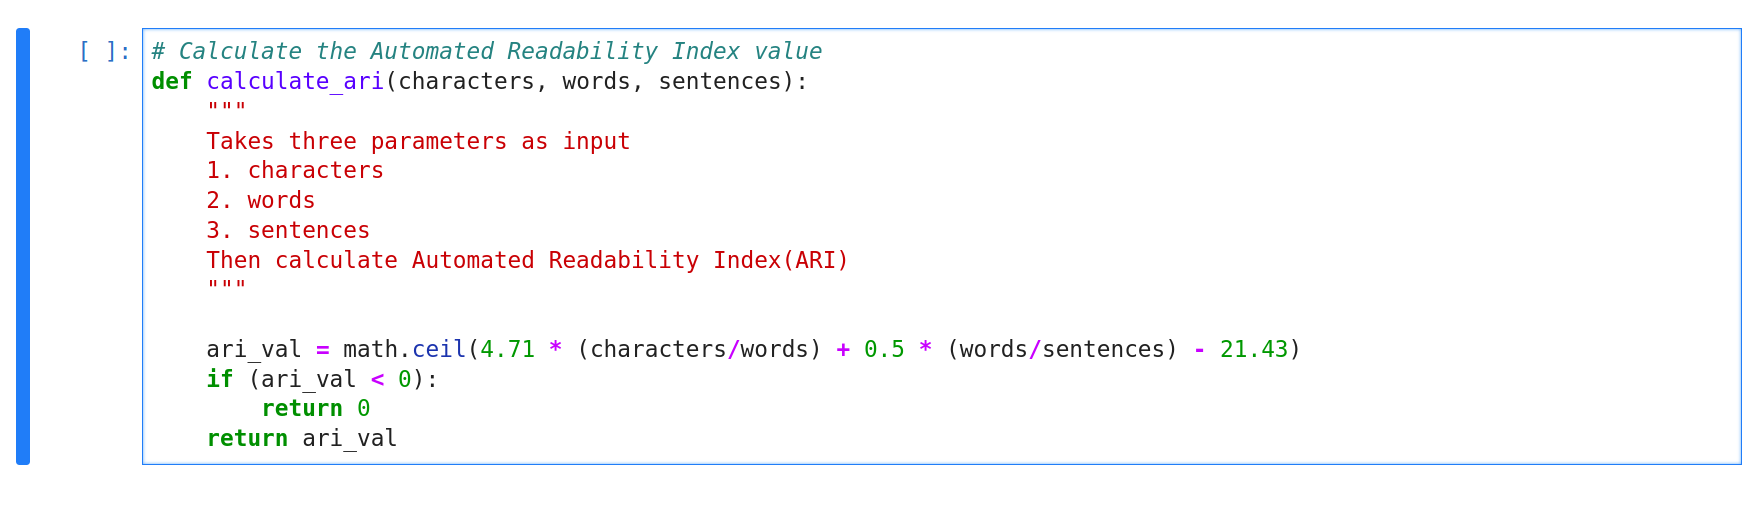
\includegraphics[scale=0.2]{screenshots/ai_a1-4.png}
\caption{\label{fig:python_code_calcualte_ari}Python code for calculating ARI}
\end{figure}

\subsection{Get Files Function}
This function will return all those file whose Automated Readability Index(ARI) need to be calculated based on the user input.

Python code of Get Files is shown in figure 5.

\begin{figure}
\centering
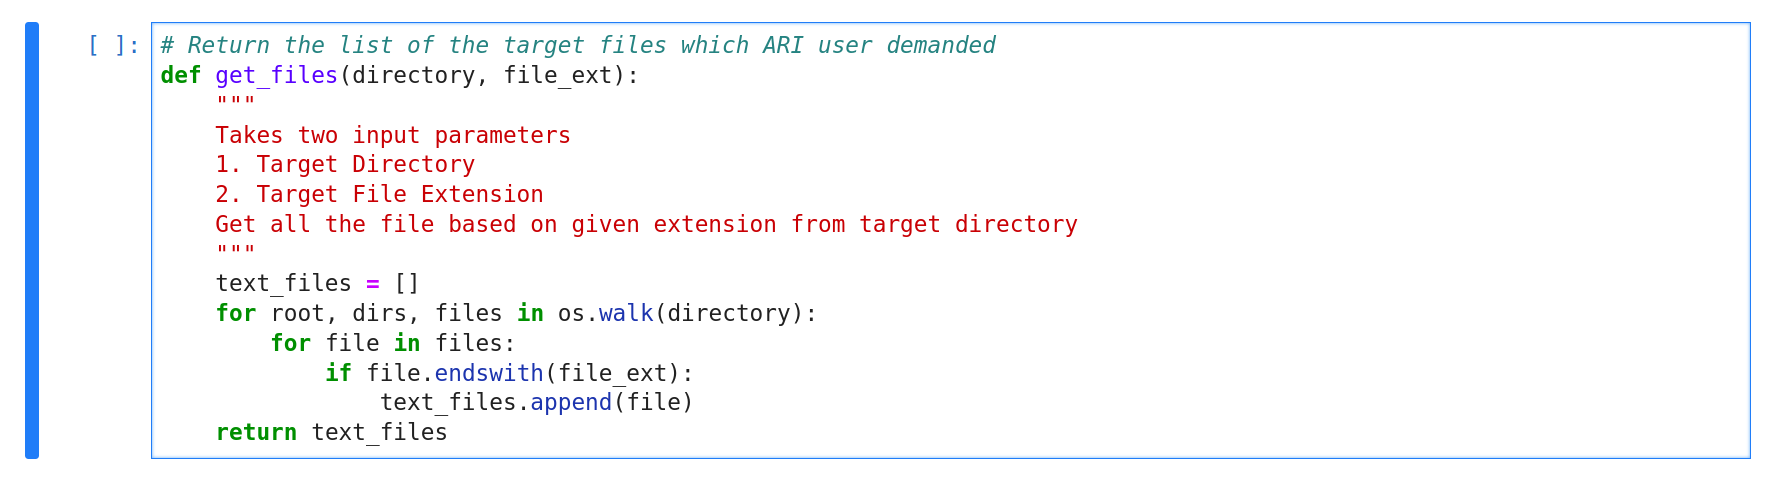
\includegraphics[scale=0.2]{screenshots/ai_a1-5.png}
\caption{\label{fig:python_code_get_files}Python code to get files}
\end{figure}

\subsubsection{Explanation of Get Files code}

The get files function take directory name and file extension as a function parameter. I have used walk function of os library that will return all the files of a given directory and then I have filtered out only those files whose extension match with the user given extension and at the end returned list of all the files whose ARI user wants to be calculated.


\subsection{Print Output function}
This function will be going to show user the result. 

Python code of Get Files is shown in figure 6.

\begin{figure}
\centering
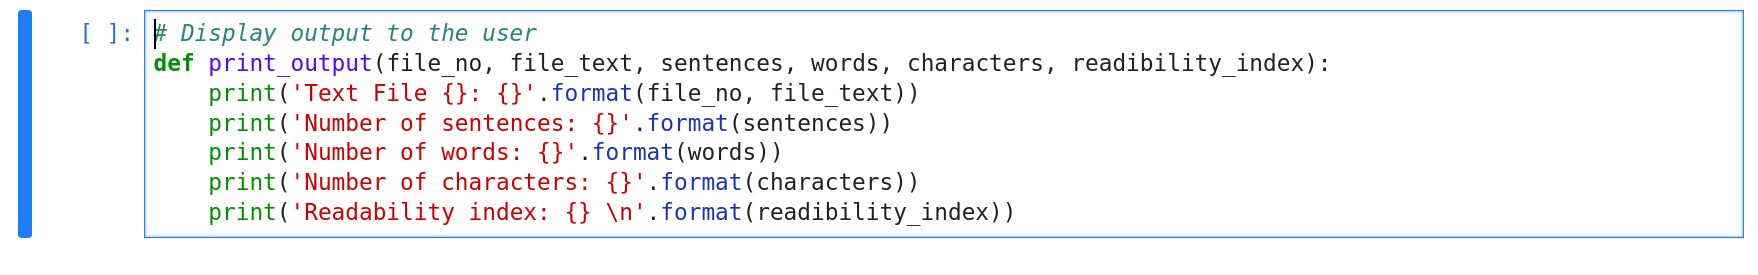
\includegraphics[scale=0.2]{screenshots/ai_a1-6.png}
\caption{\label{fig:python_code_print_output}Python code to print output}
\end{figure}



\subsection{Read Files Function}
This function will be going to read all the files whose ARI user wants. Target files will be returned from get files function that whose code I have explained in the previous section.

Python code of Read Files is shown in figure 7.

\begin{figure}
\centering
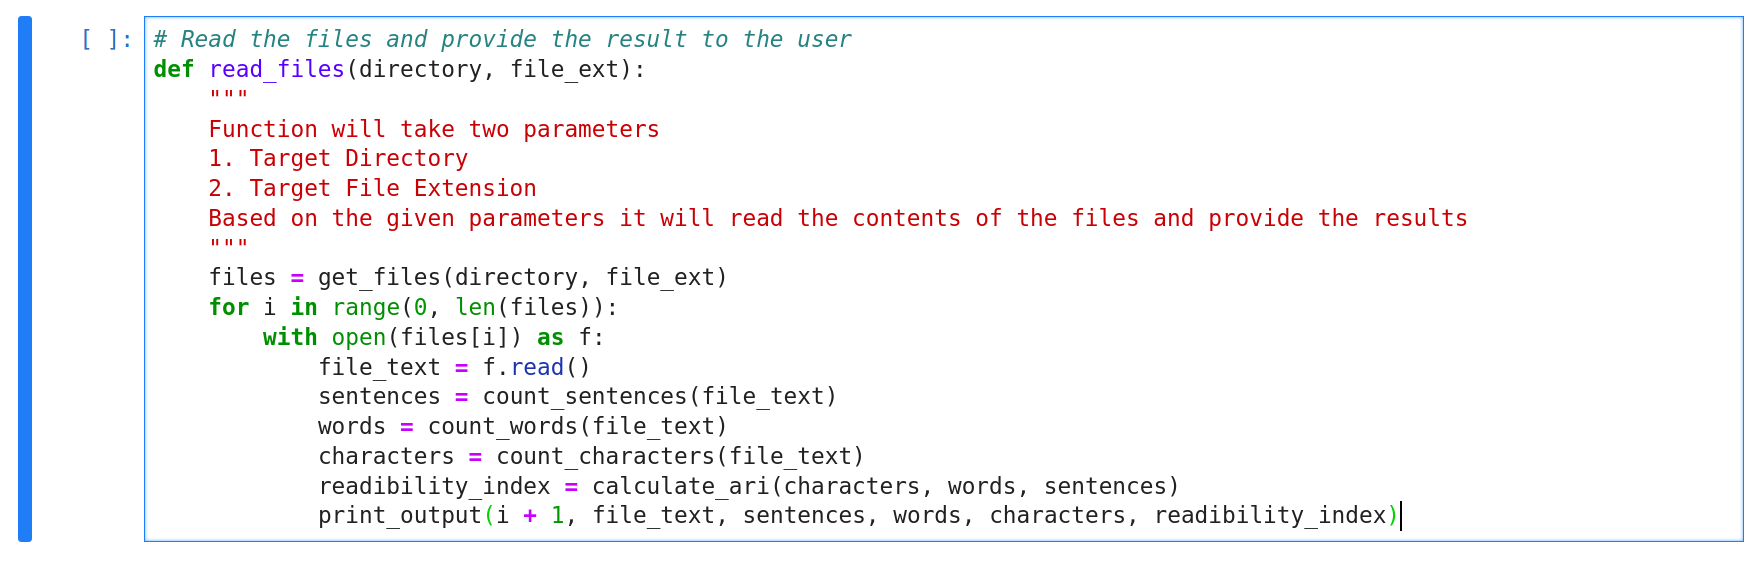
\includegraphics[scale=0.2]{screenshots/ai_a1-7.png}
\caption{\label{fig:python_code_read_files}Python code to read files}
\end{figure}

\subsubsection{Explanation of Read Files code}

This function will be going to take target directory name and file extension as a function paramters. Then with the help of get files function target files whose ARI user wants will be accquired. The algorithm of read files function is given below:

\begin{enumerate}
  \item Traverse the files list(contain the files returned by get files function).
  \item Open one by one all the files in read mode
  \item Then calculate no of words, no of characters, no of sentences and Automated Readability Index (ARI) using the functions defined above.
  \item Pass these values to the print output function that will be going to show the result.
  \item Keep iterating this process for all the target files returned by get files function.
\end{enumerate}



\subsection{Connecting with Google Drive from Google Colab}

After running this code on google colab you will be connected with google drive and you can read files from the google drive and do operation on them. The last line will be going to create a folder called 'Colab Notebooks' in the google drive and all the notebooks will be going to saved there. Then you can try getcwd function provided by os library your current directory will be that. 


Python code For connecting with google drive is shown in Figure 8.

\begin{figure}
\centering
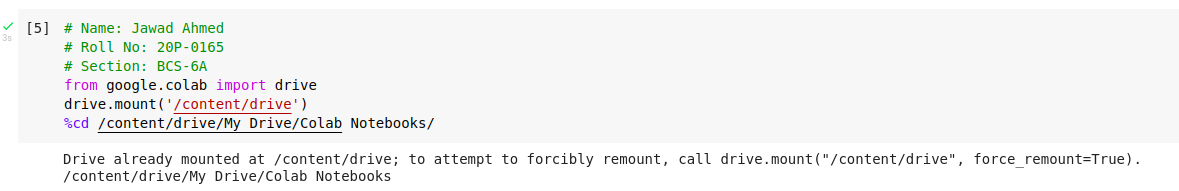
\includegraphics[scale=0.2]{screenshots/ai_a1-8.png}
\caption{\label{fig:python_code_read_files}Python code to connect google colab with google drive}
\end{figure}

\subsection{Testing the Code on the files Placed in the Google drive}
In the previous step we successfully connected with the google drive. In the google drive a folder created named 'Colab Notebooks' and in that I have placed three text files having same content as given in the given assignment document. To get your current working directory use getcwd function provided by os library. 

Colab Notebooks directory content is shown in Figure 9.

Testing Code and result is shown in Figure 10.




\begin{figure}
\centering
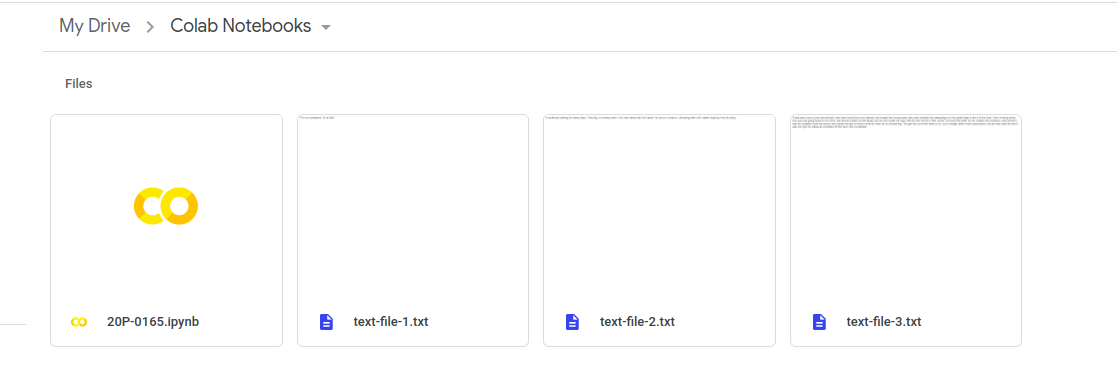
\includegraphics[scale=0.2]{screenshots/ai_a1-9.png}
\caption{\label{fig:python_code_read_files_produce_output}Content of Colab Notebooks directory}
\end{figure}


\begin{figure}
\centering
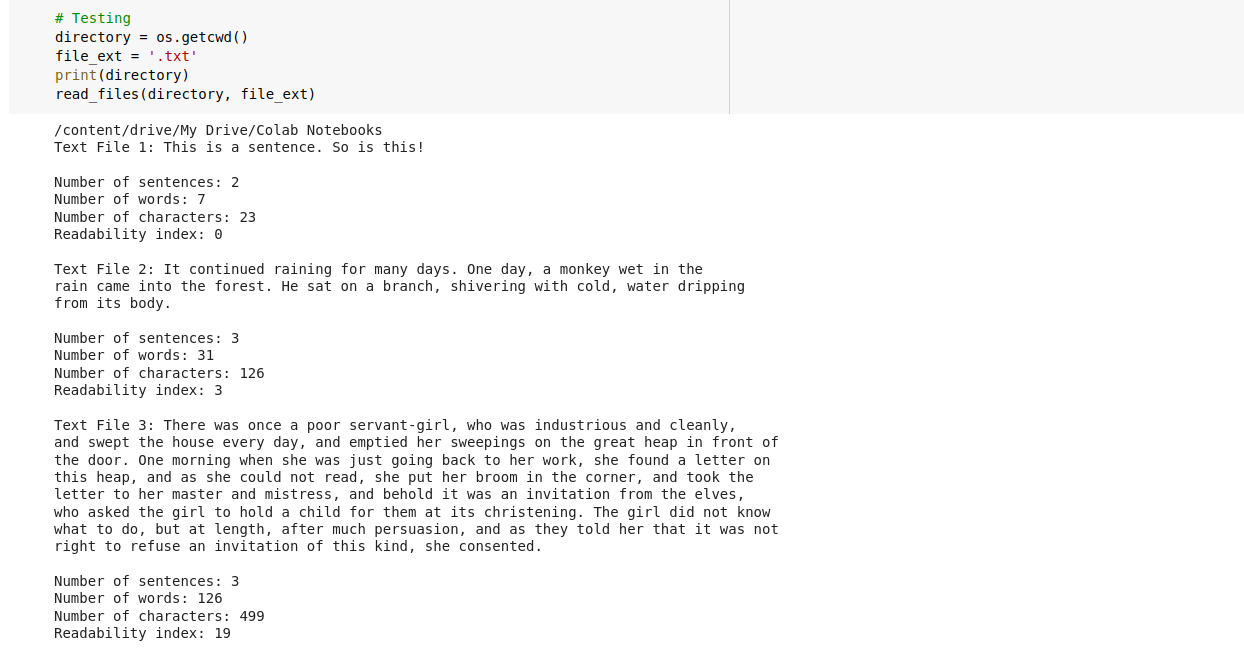
\includegraphics[scale=0.2]{screenshots/ai_a1-10.png}
\caption{\label{fig:python_code_read_files_produce_output}Result}
\end{figure}




\end{document}